\section{Observation-modality extensions (Lift)}
\label{sec:perception}

Both extensions replace the privileged object pose by sensor observations, each under its
own freeze committed before its first training launch. They share Lift's demonstrations,
split, proprioception, action encoding, diffusion head and horizons. Neither is compared
causally with Level~1: the Level~1 families trained longer on a CPU, received
\rf{train.trials} tuning trials each (the extensions received none), and saw the exact object
pose, so a Level~1 number placed beside an extension's number on the same starts is context,
not a comparison. Figure~\ref{fig:renders} shows the scenes and the point cloud.

\begin{figure}[t]
\centering
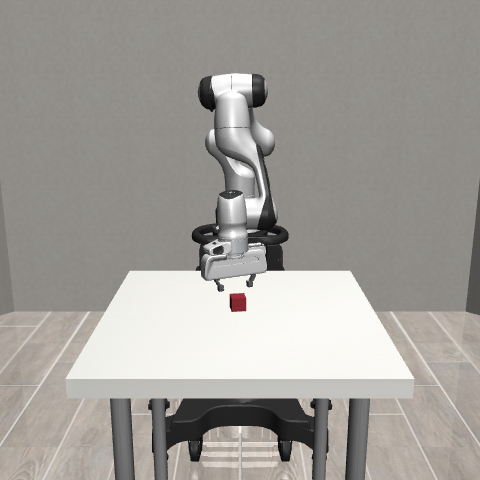
\includegraphics[width=0.32\linewidth]{generated/figures/render_lift.png}\hfill
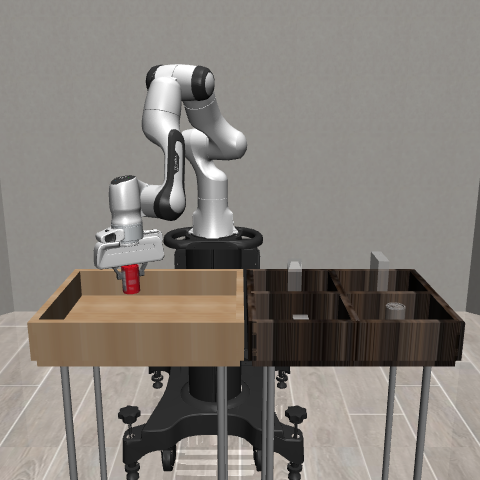
\includegraphics[width=0.32\linewidth]{generated/figures/render_can.png}\hfill
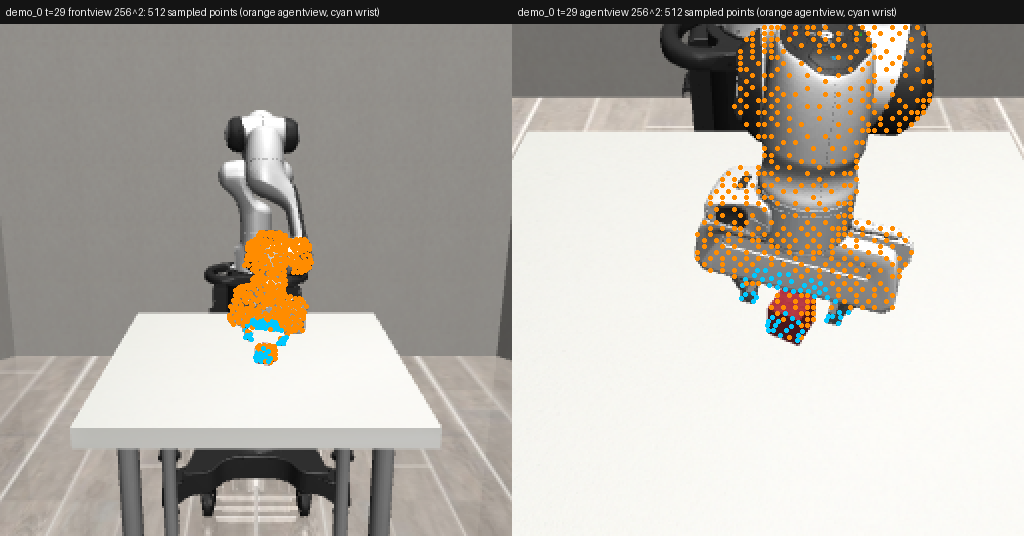
\includegraphics[width=0.32\linewidth]{generated/figures/render_pc_overlay.png}
\caption{Illustrations, not selected for outcome. Left and centre: MuJoCo renders of recorded
held-out states of the Lift and Can diffusion policies (first training seed, first held-out
start; both episodes succeeded), regenerated from the stored simulator state. Right:
the \rf{pc.points} sampled points of one Lift demonstration frame, projected onto the
camera images.}
\label{fig:renders}
\end{figure}

\subsection{RGB study: visual BC versus visual diffusion}
Table~\ref{tab:rgb} gives the result. Both arms are saturated on the Lift held-out starts:
visual diffusion succeeds on \rf{rgb.rgbdiff.k} of \rf{rgb.rgbdiff.n} episodes and visual
BC-chunk on \rf{rgb.rgbbc.k}. The preregistered difference, \rf{rgb.diff-bc.d}\,pp
[\rf{rgb.diff-bc.lo}, \rf{rgb.diff-bc.hi}], is not separated, and the seed-level interval
agrees ([\rf{sens.rgb.diff-bc.lo}, \rf{sens.rgb.diff-bc.hi}]). With both arms at or near
\rf{proto.nstates} of \rf{proto.nstates} per seed, this test cannot distinguish them; a
harder task or set would be needed. Under saturation, checkpoint selection was decided mostly
by sub-step differences in mean first-success step among checkpoints that all succeeded on
every validation start, so it carried little information.

\begin{table}[t]
\centering\small
\caption{RGB study, Lift held-out: per-checkpoint results and the preregistered difference.}
\label{tab:rgb}
% Generated by scripts/paper_assets.py (DECISIONS D-094). Do not edit.
% Sources (path sha256):
%   reports/session8/rgb_results/results.json 57663b81aafc70e9c1d850322b6bb1b894f7dad0d082976b1f546475a601390e
\begin{tabular}{lrrrll}
\toprule
Family & Seed & Step & $k/n$ & Wilson / bootstrap 95\,\% & First success / per seed \\
\midrule
Visual BC-chunk & 0 & 5,000 & 49/50 & [89.5, 99.6] & 42.8 \\
Visual BC-chunk & 1 & 5,000 & 50/50 & [92.9, 100.0] & 42.2 \\
Visual BC-chunk & 2 & 55,000 & 50/50 & [92.9, 100.0] & 44.7 \\
Visual diffusion & 0 & 55,000 & 50/50 & [92.9, 100.0] & 44.5 \\
Visual diffusion & 1 & 55,000 & 50/50 & [92.9, 100.0] & 44.3 \\
Visual diffusion & 2 & 60,000 & 50/50 & [92.9, 100.0] & 44.1 \\
\midrule
Visual BC-chunk & all &  &  & 99.3 [96.0, 100.0] & 98.0, 100.0, 100.0 \\
Visual diffusion & all &  &  & 100.0 [100.0, 100.0] & 100.0, 100.0, 100.0 \\
\multicolumn{6}{l}{Visual diffusion $-$ Visual BC-chunk: \ensuremath{+}0.7 pp [\ensuremath{+}0.0, \ensuremath{+}4.0], not separated} \\
\bottomrule
\end{tabular}

\end{table}

\subsection{Level 2: a DP3-inspired point-cloud policy (H5)}
\paragraph{Question and design.} H5 asks whether the point-cloud diffusion policy succeeds
more often than the frozen RGB diffusion policy when the cube is placed outside the
demonstrations' placement square. The primary set is Lift cube shift, paired by start with
the robustness base starts (Section~\ref{sec:robustness}); neither arm selected anything on
either set. The set was chosen after the Level~1 robustness and RGB held-out results were
known, because the RGB held-out test was saturated and cube shift was the one implemented
perturbation that leaves the training placement; the point-cloud arm's design was fixed in
its freeze before any of its rollouts. The arm is DP3-inspired in its encoder only
(Section~\ref{sec:methods}); it is not a reproduction of DP3.

\begin{table}[t]
\centering\small
\caption{Level~2 results. Placement sets: success per arm, the declared contrasts and one
context row (point cloud minus RGB on the base starts, not declared), with the hierarchical
paired bootstrap's \rf{proto.level}\,\% interval. Held-out: secondary.}
\label{tab:level2}
\resizebox{\linewidth}{!}{% Generated by scripts/paper_assets.py (DECISIONS D-094). Do not edit.
% Sources (path sha256):
%   reports/session9/level2_results/results.json 1d33c975e49df907a6543b17e0cf36d047f7b5ce11aa69a355313e146c22571e
\begin{tabular}{llll}
\toprule
Arm or contrast & Set & Success \% or difference [95\,\% CI] & Per seed or outcome \\
\midrule
\multicolumn{4}{l}{\emph{Placement (validation regime; primary H5 on the cube shift)}} \\
Point-cloud diffusion & base & 100.0 [100.0, 100.0] & 100.0, 100.0, 100.0 \\
Point-cloud diffusion & cube shift & 56.7 [43.3, 70.0] & 64.0, 56.0, 50.0 \\
Visual diffusion & base & 100.0 [100.0, 100.0] & 100.0, 100.0, 100.0 \\
Visual diffusion & cube shift & 98.0 [93.3, 100.0] & 100.0, 98.0, 96.0 \\
\midrule
\textbf{H5:} point cloud $-$ RGB on cube shift &  & \ensuremath{-}41.3 [\ensuremath{-}54.0, \ensuremath{-}28.0] & separated (\ensuremath{-}) \\
drop of Point-cloud diffusion (base $-$ cube shift) &  & \ensuremath{+}43.3 [\ensuremath{+}30.0, \ensuremath{+}56.7] & separated (\ensuremath{+}) \\
drop of Visual diffusion (base $-$ cube shift) &  & \ensuremath{+}2.0 [\ensuremath{+}0.0, \ensuremath{+}6.7] & not separated \\
point cloud $-$ RGB on base &  & \ensuremath{+}0.0 [\ensuremath{+}0.0, \ensuremath{+}0.0] & not separated \\
drop point cloud $-$ drop RGB &  & \ensuremath{+}41.3 [\ensuremath{+}28.0, \ensuremath{+}54.0] & separated (\ensuremath{+}) \\
\midrule
\multicolumn{4}{l}{\emph{Held-out (secondary; RGB records reused, never rerun)}} \\
Point-cloud diffusion & held-out & 100.0 [100.0, 100.0] & 100.0, 100.0, 100.0 \\
Visual diffusion & held-out & 100.0 [100.0, 100.0] & 100.0, 100.0, 100.0 \\
point cloud $-$ RGB, success &  & \ensuremath{+}0.0 [\ensuremath{+}0.0, \ensuremath{+}0.0] & not separated \\
point cloud $-$ RGB, censored length (steps) &  & \ensuremath{+}1.1 [\ensuremath{-}1.4, \ensuremath{+}3.4] & not separated \\
\bottomrule
\end{tabular}
}
\end{table}

\begin{figure}[t]
\centering
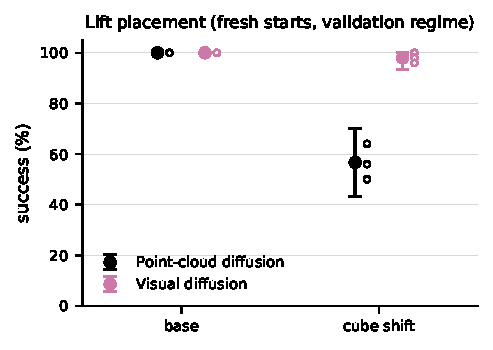
\includegraphics[width=0.8\linewidth]{generated/figures/level2.pdf}
\caption{Level~2: success of the point-cloud and RGB diffusion arms on the base starts and
under cube shift, with per-seed values.}
\label{fig:level2}
\end{figure}

\paragraph{Result.} The answer is no, in the opposite direction
(Table~\ref{tab:level2}, Figure~\ref{fig:level2}). Both arms succeed on every base start.
Under cube shift the point-cloud arm falls to \rf{l2.pcdiff.cube.succ}\,\% while the RGB arm
keeps \rf{l2.rgbdiff.cube.succ}\,\%; H5's difference is \rf{l2.h5.d}\,pp [\rf{l2.h5.lo},
\rf{l2.h5.hi}], separated, and the seed-level interval agrees ([\rf{sens.l2.h5.lo},
\rf{sens.l2.h5.hi}]). The point-cloud arm's own drop (\rf{l2.pcdiff.drop.d}\,pp) is separated
and the RGB arm's (\rf{l2.rgbdiff.drop.d}\,pp) is not. Because both arms are at the ceiling on
the base starts, the difference of drops equals H5 with its sign reversed and adds no
information. The point-cloud arm's failures are mostly misses next to the displaced cube and drops
(Table~\ref{tab:taxonomy}). On the held-out starts both arms succeed on every episode, so that
secondary comparison is uninformative; it is a check that the point-cloud arm works in
distribution, not evidence of equivalence.

\paragraph{What the result does and does not show.} H5 compares two complete policies, not
two modalities. Besides the input, the arms differ in their encoders (a ResNet-18 per camera,
\rf{rgb.enc.params} encoder parameters in total, against \rf{pc.enc.params} for the point
encoder), in augmentation (random crops for RGB, none for the cloud), and in the frame of the
input: the cloud is in absolute world coordinates, so shifting the cube moves its points to
coordinates the encoder never saw during training, whereas a convolutional encoder with
random crops may be more tolerant of translation (not tested here). The depth is noise-free and the calibration
exact. The result is therefore that \emph{this} point-cloud package, trained on
\rf{data.lift.train} demonstrations without augmentation, generalizes worse to unseen cube
positions than the matched RGB package. It does not test, and should not be read as
contradicting, the generalization results reported for DP3~\citep{ze2024dp3} under its own
design and tasks.
